% ======================================================================
% doc_body.tex -- the main document content.
%
% This template is for UNCG's PHY 419 (Advanced Lab) course,
% Assignment 1: Research Proposal.
%
% Adapted from the APS REVTeX 4.2 template in Overleaf on 2019-08-20.
%
% This file is part of the APS files in the REVTeX 4.2 distribution.
%     Version 4.2a of REVTeX, December 2014
%     Copyright (c) 2014 The American Physical Society.
%     See the REVTeX 4 README file for restrictions and more information.
%
% Using this requires BibTeX. Overleaf handles this automatically,
% **if** you have the right files in your project folder (*.bib),
% and you recompile both this document and the *.bib document after
% making changes to what's in *.bib.
%
% Note that the comment character "%" has been used to deactivate
% certain lines below, but keep the code in the file in case you want
% to reactivate them at some point.% to reactivate them at some point.


%
% ======================================================================
\documentclass[%
 reprint,
 11pt,
 amsmath,amssymb,
 aps,
]{revtex4-2}

\usepackage{graphicx}% Include figure 
\newcommand{\panel}[2]{\begin{tabular}[b]{@{}l@{}}\textbf{(#1)}\\[1pt]#2\end{tabular}}
\usepackage{dcolumn}% Align table columns on decimal point
\usepackage{bm}% bold math
\usepackage{hyperref}% enables hyperlinks in the PDF
\usepackage{subcaption}

% --- Compact layout for 11pt ---
\usepackage[letterpaper, top=0.6in, bottom=0.7in,
            left=0.6in, right=0.6in, columnsep=0.25in]{geometry}
\linespread{0.97}                         % slightly tighter lines, still readable

% Less white space around figures and floats
\setlength{\textfloatsep}{8pt plus 2pt minus 2pt}
\setlength{\floatsep}{6pt plus 2pt minus 2pt}
\setlength{\dbltextfloatsep}{8pt plus 2pt minus 2pt}   % for figure*
\setlength{\dblfloatsep}{6pt plus 2pt minus 2pt}
\setlength{\abovecaptionskip}{4pt}
\setlength{\belowcaptionskip}{0pt}

% Tighter reference list
\setlength{\bibsep}{0pt plus 0.3ex}

\begin{document}

\title{Quantifying Expansion Anisotropy in Osmotic and Tensile Expansion Microscopy: A Comparison of MAGNIFY and TExM}% Force line breaks with \\

\author{Tejasvin Shrikanth} % Student
  \email{txs712@case.edu}

\author{Vignesh Venkataramani} % Research mentor
  \email{vxv189@case.edu}

\author{Lydia Kisley} % Research mentor
  \email{lxk284@case.edu}
\affiliation{%
 Department of Physics\\
 Case Western Reserve University, Cleveland, Ohio 44106, USA
}%

\date{\today}% It is always \today, today,
             %  but any date may be explicitly specified

\begin{abstract}
Expansion microscopy (ExM\cite{exm}) achieves super-resolution imaging by embedding a biological specimen in a hydrogel and physically enlarging it, so that features below the diffraction limit become separable under an ordinary light microscope. This process relies on the assumption that the sample expands isotropically, preserving structure and shape so that nanoscale dimensions can be scaled directly by the expansion factor. Two distinct approaches can achieve this expansion: osmotic swelling (as used in protocols such as MAGNIFY\cite{magnify}), which relies on charge repulsion and osmotic pressure in water; and tensile expansion (TExM\cite{texm}), which mechanically stretches a hydrogel using a custom expansion device. This project will quantify and compare the magnitude and spatial structure of anisotropy in both osmotic and tensile expansion. Two-photon polymerized fiducial markers, printed using direct laser writing (Nanoscribe), are transferred into the hydrogel at gelation to provide a reference of known geometry against which local deformation is measured before and after expansion. Self-identifying ArUco markers allow correspondence to be established automatically rather than by manual landmark placement. The recovered marker coordinates are compared against an ideal similarity transform, with the resulting deviations yielding a map of local and large-scale anisotropy. These deviations will be characterized by their magnitude, orientation and spatial correlation, and each will be tracked through the course of expansion. Finally, cells will be expanded alongside the markers under different homogenization conditions to evaluate how homogenization influences anisotropy, contrasting the mechanical fidelity of osmotic swelling with tensile expansion.


\end{abstract}

\maketitle
% ========================================================================

\section{Introduction \& Background}

\subsection{Expansion Microscopy}

Light microscopy is a central tool for the study of biological structure. Due to the fundamental physical restriction of the diffraction limit of light, the resolution of optical microscopy is limited to $\lambda/2\mathrm{NA}$ or roughly 250~nm.\cite{abbe} Many structures that determine biological function lie below this scale, including the nanoscale organization of synaptic proteins, nuclear pores, membrane protein clusters and cytoskeletal filaments.\cite{xu2013actin,schermelleh} Super-resolution techniques overcome this limit either through specialized modifications to the optical hardware, as in STED and linear SIM,\cite{sted,sim} or through computationally intensive analysis of many raw images, as in PALM/STORM and SOFI.\cite{palm,storm,sofi} Both approaches require dedicated instruments, specific fluorophores and expert operation, which limits their accessibility.\cite{schermelleh} Expansion microscopy (ExM) instead embeds a specimen in a hydrogel and physically enlarges it, so that features below the diffraction limit become distinguishable under an ordinary microscope, reaching approximately 70~nm resolution at 4.2-fold expansion\cite{exm} and 25~nm at ten-fold.\cite{magnify}

In osmotic ExM protocols, the specimen is fixed, labeled and anchored to a charged hydrogel network, then homogenized by proteinase digestion or by heat and detergent denaturation, so that its own mechanical structure does not resist expansion.\cite{proexm,magnify} On immersion in water, the network swells through osmotic repulsion,\cite{exm,jcs} and the uniformity of swelling depends strongly on the homogenization protocol. Inadequately homogenized specimens may crack or expand incompletely.\cite{gao,magnify} TExM, a technique developed in our lab, instead uses its own tough double-network hydrogel, stretched mechanically by an iris-like device whose nine arms grip the gel at its edge, permitting precise and repeatable expansion up to 4.2-fold.\cite{texm} Whereas osmotic swelling expands the gel in all three dimensions, tensile expansion acts only within the plane of the gel, so the specimen is enlarged laterally while its thickness is unchanged or, by the Poisson effect, reduced.\cite{texm} Fixed-cell TExM protocols still include proteinase K digestion, but since strain enters through the grips rather than arising throughout the volume, the TExM deformation field may be non-uniform in ways that osmotic swelling is not.\cite{texm}

\subsection{Distortion and Anisotropy in Imaging}

Expansion microscopy rests on the assumption that the specimen expands nearly isotropically and homogeneously, so that every distance is enlarged by the same intrinsic factor irrespective of direction or position, and true dimensions may be recovered from a single expansion factor, $\lambda$.\cite{exm,jcs}

In practice, expansion departs measurably from this ideal, with published protocols reporting distortions of typically 1\% to 4\%.\cite{exm,proexm,magnify} Incomplete homogenization may leave residual structure that resists swelling,\cite{gao,magnify} heterogeneity in the gel network may render swelling non-uniform,\cite{gelmap} and the mechanism driving expansion determines where strain originates.\cite{texm}

Several approaches have been developed to measure this distortion, each comparing a reference before and after expansion (Fig.~\ref{fig:references}). Most protocols, including MAGNIFY, image the same intrinsic biological structures in both states (Fig.~\ref{fig:references}a), register the images using a similarity transform (rotation, translation and uniform scaling), and report the residual as a root-mean-square length error.\cite{magnify} pan-ExM additionally compared a similarity model with an affine model, which also permits shear and unequal scaling, and found that the error fell from approximately 3\% to 1.6\%, attributing roughly half of the distortion to anisotropic stretching.\cite{panexm} Other methods introduce an extrinsic reference of known geometry into the gel: GelMap transfers a lithographically patterned protein grid, from which a local expansion factor may be derived for each grid square (Fig.~\ref{fig:references}b),\cite{gelmap} while TExM embeds rigid fluorescent markers printed by two-photon polymerization, matched manually before and after expansion to yield a single global distortion value (Fig.~\ref{fig:references}c).\cite{texm}
\begin{figure}[t]
    \centering
    \panel{a}{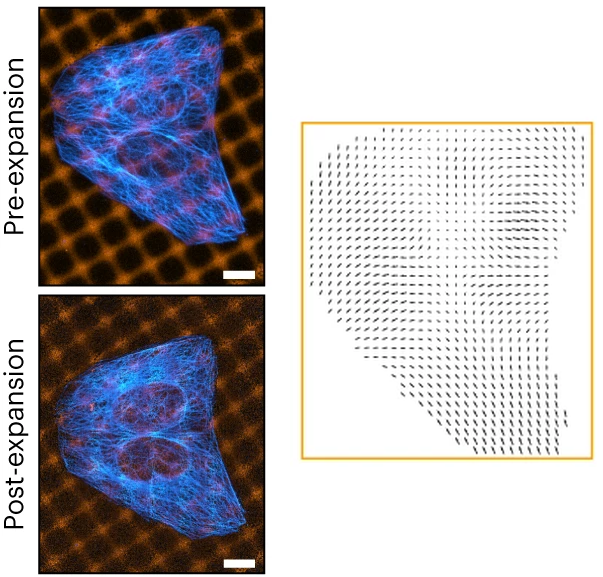
\includegraphics[height=0.355\columnwidth]{figures/panel_a_intrinsic.png}}\hfill
    \panel{b}{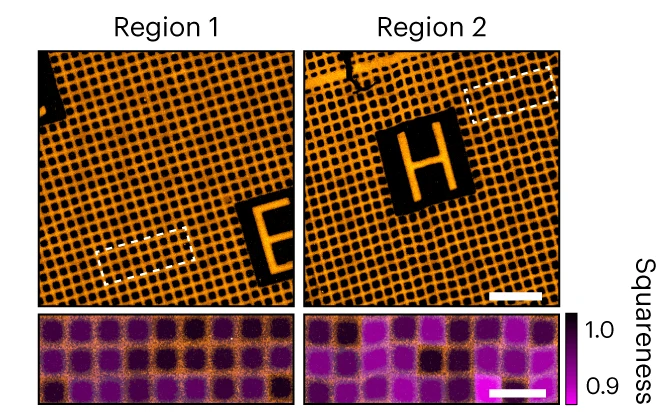
\includegraphics[height=0.355\columnwidth]{figures/panel_b_gelmap.png}}\\[6pt]
    \panel{c}{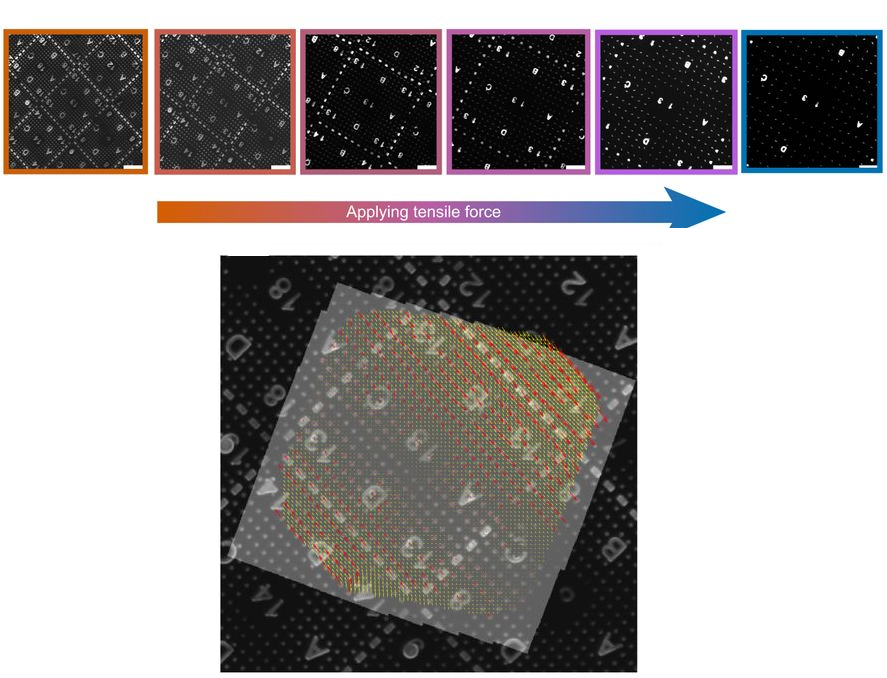
\includegraphics[width=0.65\columnwidth]{figures/panel_c_texm.png}}
    \caption{\textbf{Intrinsic and extrinsic references used to measure expansion distortion.}
    (a) Intrinsic reference: a cell imaged before and after expansion (microtubules, blue),
    and the deformation field obtained by registering the two images of its microtubule
    cytoskeleton. (b) Extrinsic protein reference: two regions of an expanded,
    lithographically patterned protein grid, with local deformation of each square
    colour-coded by the squareness metric. (a,b) Adapted from Damstra et al.,
    Fig.~2a,c,e,~\cite{gelmap} under CC BY 4.0.
    (c) Extrinsic printed reference: two-photon-printed fluorescent markers after tensile
    expansion, registered to the pre-expansion pattern by a similarity transform, with
    residual mismatch (red) and interpolated deformation field (yellow).
    Adapted from Venkataramani et al., Fig.~2e.~\cite{texm}}
    \label{fig:references}
\end{figure}


These registration and fiducial-marker approaches are, however, specific to the protocols for which they were developed. Each employs its own reference, model and metric, and none has been applied across both osmotic and tensile expansion, so that reported values cannot be compared directly between techniques. Some are further constrained by the chemistry they measure: GelMap's protein grid is itself subject to homogenization,\cite{gelmap} and registration against biological structure is confined to regions where recognizable, well-labelled features exist.\cite{exm,proexm,magnify}

Moreover, existing methods quantify the extent of distortion without characterizing its nature. Similarity-based registration absorbs direction-dependent stretch into a single residual,\cite{exm,proexm,magnify} GelMap's shape metric combines stretch and skew into one value,\cite{gelmap} and pan-ExM did not characterize the anisotropic component it identified.\cite{panexm} It therefore remains unknown how expansion distortion is distributed by direction and by position, over what length scale it is correlated, and whether osmotic and tensile expansion give rise to distinct modes of distortion.

\section{Objectives}
To address these questions, this project will quantify and characterize the magnitude and spatial structure of expansion distortion in osmotic expansion (MAGNIFY\cite{magnify}) and tensile expansion (TExM\cite{texm}).

\textbf{Objective 1:} Printed reference markers in MAGNIFY and TExM hydrogels (end of fall semester). Design and print a self-identifying fluorescent marker pattern, transfer it into both hydrogels, and confirm that the markers remain anchored and fluorescent before, during and after expansion. Acquire expansion series in both systems before the laboratory closure.

\textbf{Objective 2:} Analysis pipeline with quantitative distortion metrics (spring break). Extend the marker detection pipeline to measure local deformation and separate it into anisotropy, inhomogeneity and local warping, establish the smallest distortion the method can detect, and apply it to compare both techniques across expansion factor.

\textbf{Objective 3:} MAGNIFY and TExM with cells (end of senior year). Expand cells alongside the marker pattern in both systems and use the measured deformation fields to assess how faithfully each technique preserves nanoscale cellular structure, including a direct comparison at a matched expansion factor. A shortened digestion will be compared with the standard protocol to evaluate how homogenization influences anisotropy.

\section{Significance and Justification}

Expansion microscopy has become a widely used means of achieving super-resolution on conventional microscopes, and is increasingly applied in biomedical research, including studies of disease.\cite{jcs,magnify} Because every measurement made with the technique is converted to true dimensions using a single expansion factor, it is critical that expansion faithfully preserves the geometry of the specimen.\cite{exm} While existing protocols have been validated to within a few percent,\cite{exm,proexm,magnify} it is nevertheless important to understand how the remaining distortion is structured, since the length scale over which it varies determines how densely a specimen must be referenced for it to be corrected.\cite{gelmap} Characterizing this structure, and determining whether it differs between osmotic and tensile expansion, would offer guidance on the limits of expansion microscopy's accuracy as presently implemented, and on the conditions under which corrections can be trusted.

Additionally, the printed markers and openly released analysis pipeline developed here could serve as a common calibration standard applicable to any expansion protocol, including emerging techniques such as TExM that currently lack one.\cite{texm} Because the markers are not composed of protein, they could also serve as an independent reference in studies where homogenization itself is varied, including the comparison made here.\cite{gelmap}


\section{Methods}
\subsection{Fabrication and Transfer}

I will print the marker pattern by two-photon polymerization (Nanoscribe) in fluorescent resist on glass coverslips, and cast both MAGNIFY and TExM gels over them.\cite{texm} Three pass/fail tests will be carried out first in each gel: that the markers release from the glass, remain anchored to the gel, and survive that gel's processing chemistry.\cite{magnify,texm}

\subsection{Imaging and Data Collection}

Markers will be imaged by widefield fluorescence microscopy, where possible before, during and after expansion. Expansion factor will be varied through solution ionic strength in MAGNIFY\cite{magnify} and iris position in TExM,\cite{texm} and measured from the markers in each case. Datasets will include a MAGNIFY expansion series with at least three gels per condition, swelling time-lapses, control images of static gels and a known stretched elastomer, and a TExM series up to 4.2-fold.

\subsection{Analysis}

\paragraph{Marker detection.}
Markers will be detected and decoded with the ArUco module of OpenCV,\cite{aruco,opencv}
and all analysis will be carried out in Python (NumPy and SciPy\cite{numpy,scipy}),
extending an existing detection and strain-analysis pipeline. Because each marker's
identifier links it to its design position, deformation can be measured without image
registration. Analysis will be confined to single Nanoscribe write fields, since
stitching between fields could otherwise mimic distortion. The global expansion factor
will be obtained by fitting a similarity transform (uniform scaling, rotation and
translation) to all markers in a field.

\paragraph{Local deformation gradient $\mathbf{F}$.}
For each marker $i$, with design position $\mathbf{X}_i$ and measured position
$\mathbf{x}_i$, the local deformation gradient $\mathbf{F}$ will be fitted by least
squares over its $k$ nearest neighbours $j$,\cite{falk,gullett}
\begin{equation}
  \mathbf{F}_i = \arg\min_{\mathbf{F}} \sum_{j=1}^{k}
  \left\| (\mathbf{x}_j - \mathbf{x}_i) - \mathbf{F}\,(\mathbf{X}_j - \mathbf{X}_i) \right\|^2 ,
  \label{eq:F}
\end{equation}
with $k$ varied to set the length scale of the measurement.

\paragraph{Decomposition into rotation and stretch.}
$\mathbf{F}$ is then decomposed into a rotation $\mathbf{R}$ and a stretch
$\mathbf{U}$,\cite{hoger1984}
\begin{equation}
  \mathbf{F} = \mathbf{R}\,\mathbf{U}, \qquad
  \mathbf{U} = \sqrt{\mathbf{F}^{\mathsf{T}}\mathbf{F}} .
  \label{eq:polar}
\end{equation}
The eigenvalues of $\mathbf{U}$, $\lambda_1 \ge \lambda_2$, are the principal stretches. The rotation
does not distort the specimen and is discarded. Uniform, isotropic expansion
corresponds to $\mathbf{U} = \lambda\mathbf{I}$ everywhere.

\paragraph{Distortion metrics.}
Departures from uniform expansion are quantified as anisotropy, by
$A = \lambda_1/\lambda_2$; inhomogeneity, by the coefficient of variation of the local
expansion factor $\sqrt{\det\mathbf{F}}$ across the gel; and local warping, by the
residual of the fit in Eq.~\eqref{eq:F}.\cite{falk} Each will be mapped across the gel.

\paragraph{Spatial structure.}
To distinguish smooth, large-scale distortion, which can be corrected after imaging,
from local distortion, which cannot, the spatial correlation of each metric will be
measured. For the local expansion factor $\lambda(\mathbf{x}) = \sqrt{\det\mathbf{F}}$,
with fluctuation $\delta\lambda = \lambda - \langle\lambda\rangle$, the normalised
autocorrelation
\begin{equation}
  C(r) = \frac{\langle \delta\lambda(\mathbf{x})\,\delta\lambda(\mathbf{x}+\mathbf{r}) \rangle}
              {\langle \delta\lambda^2 \rangle}, \qquad r = |\mathbf{r}| ,
  \label{eq:corr}
\end{equation}
defines a correlation length $\xi_c$, taken as the distance at which $C$ falls to $1/e$;
this sets how densely a specimen must be referenced for its distortion to be corrected.
The directions of maximum stretch will also be compared across the field to determine
whether anisotropy is randomly oriented or aligned along a preferred axis. Finally,
root-mean-square length error against measurement length will be computed for comparison
with published values.
\paragraph{Detection limit.}
The smallest detectable distortion will be established from simulated deformations and
the control datasets before any comparison is made.

\subsection{Cellular Samples}
Once the markers pass the transfer tests, I will culture cells directly on the printed coverslips so that cells and markers are embedded in the same gel. Cells will be fixed, immunostained for microtubules in a channel separate from the marker dye, anchored to the gel (with AcX for TExM, and through MAGNIFY's own chemistry), and homogenized before expansion, using each technique's standard protocol and a shortened digestion for comparison. Cells and the surrounding markers will be imaged in the same fields of view before and after expansion. Comparing the local expansion of each cell with the marker-derived deformation field at the same location will show how closely cellular structure follows the gel, and how much of the distortion seen in a biological sample arises from the gel itself rather than from the specimen.


\subsection{Potential Problems}

The principal risk is that the markers fail one of the transfer tests: release from the glass, anchoring to the gel, or survival of the processing chemistry. Marker anchoring can be improved by silanization of the printed features, alternative dyes can be substituted if fluorescence does not survive, and a second print session will be reserved in case printing itself fails. If in-situ imaging during expansion proves impractical, the study will rely on images taken at equilibrium, and the question of equilibration time will be set aside.

\section{Expected results}

Since osmotic protocols report root-mean-square length errors of 1 to 4\% of the measured distance, for distances of roughly ten to a few hundred micrometres,\cite{exm,panexm,magnify} and since pan-ExM attributed roughly half of its error to direction-dependent stretch,\cite{panexm} I anticipate a measurable and structured departure from uniform scaling in MAGNIFY\cite{magnify} rather than purely random noise. Homogenization is likely to play a central role: where it leaves residual structure in the specimen, swelling is resisted locally,\cite{gao,magnify} so I expect expansion to vary with position and, where that structure is oriented, with direction. Because the two techniques differ in how, and how far, the specimen is homogenized, and in where strain originates,\cite{magnify,texm} I anticipate that they will distort in different ways: MAGNIFY through short-range variation tied to the specimen and gel, and TExM through larger-scale, direction-dependent stretch radiating from the nine grips at the gel's edge. However, I do not anticipate large distortions in either case. TExM reports distortions below 12\,$\mu$m across 1.3\,mm$^2$,\cite{texm} and pilot data show the local expansion factor varying by a coefficient of variation of only 1 to 3\%. I therefore expect anisotropy of a few percent at most ($A \lesssim 1.05$) and comparable variation in local expansion, with distortions exceeding about 10\% confined to visibly damaged regions such as tears. Since the estimated detection limit of the method lies well below 1\%, departures of this size should be clearly resolvable.

\begin{acknowledgments}
I would like to thank Lydia Kisley and Vignesh Venkataramani for their guidance and mentorship.
\end{acknowledgments}



\section{References}

\bibliography{bibfile}% Produces the bibliography via BibTeX.

\end{document}

%%%%%% End of file doc_body.tex %%%%%%

% ========================================================================